\chapter{R programming}

\href{https://class.coursera.org/rprog-016/}{Coursera} classes

{\it Programming with Data} by John Chambers - originally was the \texttt{S} language: \texttt{R} is a ``dialect'' of \texttt{S}. 
{\it Software for Data Analysis} by John Chambers (Springer, 2008)

Assignement operator: \href{http://stackoverflow.com/questions/1741820/assignment-operators-in-r-and}{stackoverflow}


\begin{lstlisting}
> x <- c(3, 5, 1, 10, 12, 6)
> x[x %in% 1:5] <- 0
\end{lstlisting}


\begin{figure}[htb]\begin{center}
\subfigure[]{\label{fig:types}
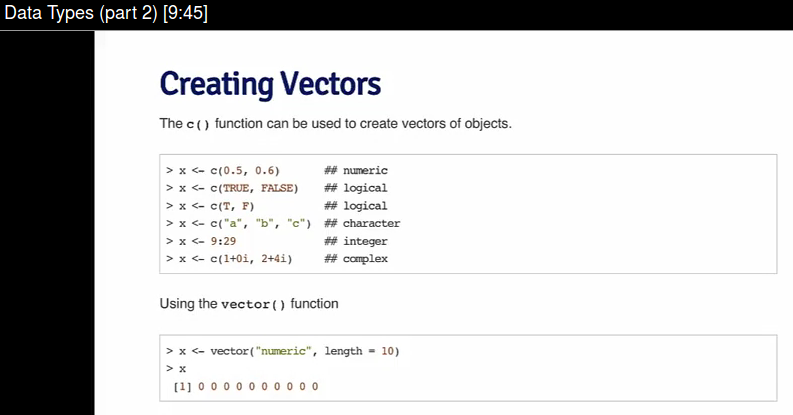
\includegraphics[width=0.45\textwidth]{01_rprogramming/pics/data_types.png}}
\subfigure[]{\label{fig:matrix}
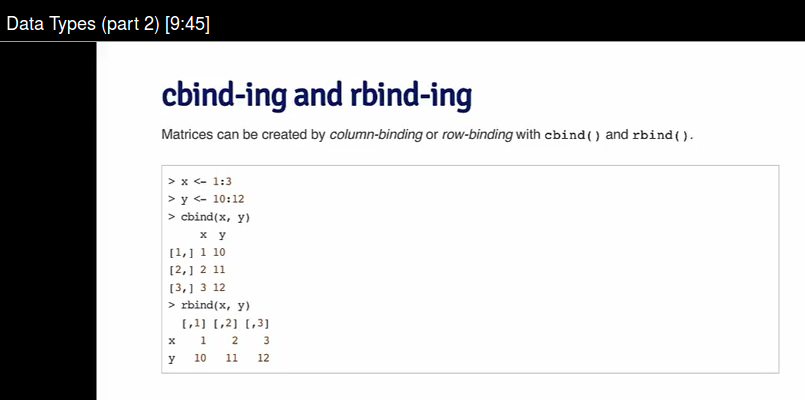
\includegraphics[width=0.45\textwidth]{01_rprogramming/pics/matrixbind.png}}
\caption{(a) Available data types: numerical, integer (1 = numerical, 1L = integer), complex, logical, character. Single elements are vector! (b) Build matrices binding
vectors as rows or columns.}
\end{center}\end{figure}



\begin{figure}[htb]\begin{center}
\subfigure[]{\label{fig:lists}
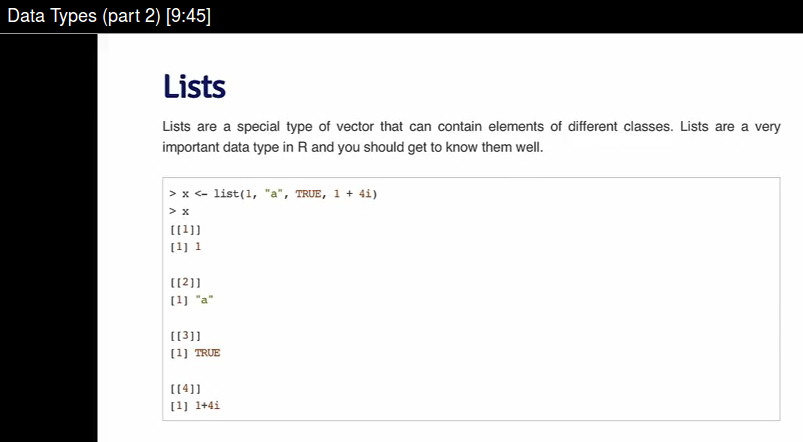
\includegraphics[width=0.45\textwidth]{01_rprogramming/pics/lists.png}}
\subfigure[]{\label{fig:factors}
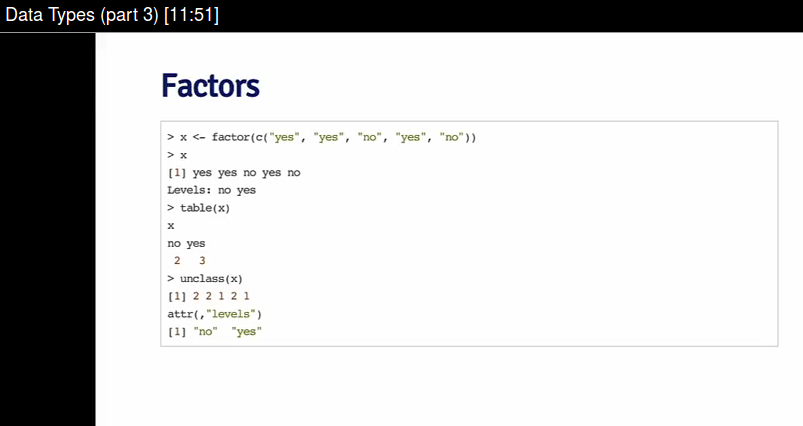
\includegraphics[width=0.45\textwidth]{01_rprogramming/pics/factors.png}}
\caption{(a) Vectors element are always of the same type, eventually the type is re-assigned. Lists can contain different types, are accessed with $[[]]$. 
(b) Factors represent {\bf categorical data} and basically label integer flags. Levels (= list of flags) are authomatically ordered alphabetically! 
To avoid this and have the base level desired add \texttt{, levels = c(``yes'', ``no'')}}
\end{center}\end{figure}



\begin{figure}[htb]\begin{center}
\subfigure[]{\label{fig:frames}
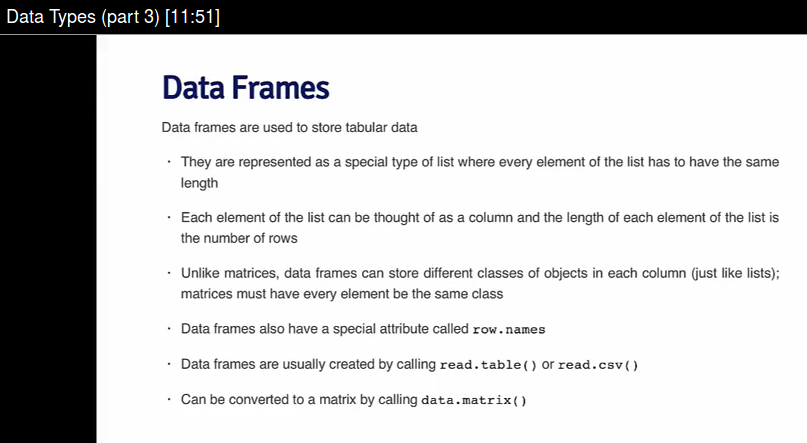
\includegraphics[width=0.45\textwidth]{01_rprogramming/pics/dataframes.png}}
\subfigure[]{\label{fig:names}
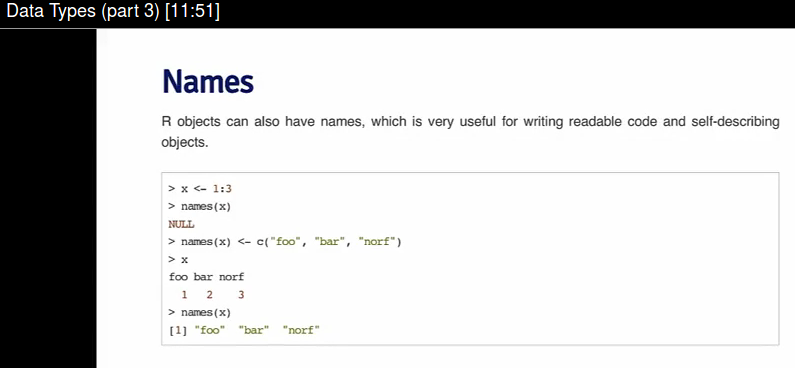
\includegraphics[width=0.45\textwidth]{01_rprogramming/pics/names}}
\caption{}
\end{center}\end{figure}


\begin{figure}[htb]\begin{center}
\subfigure[]{\label{fig:}
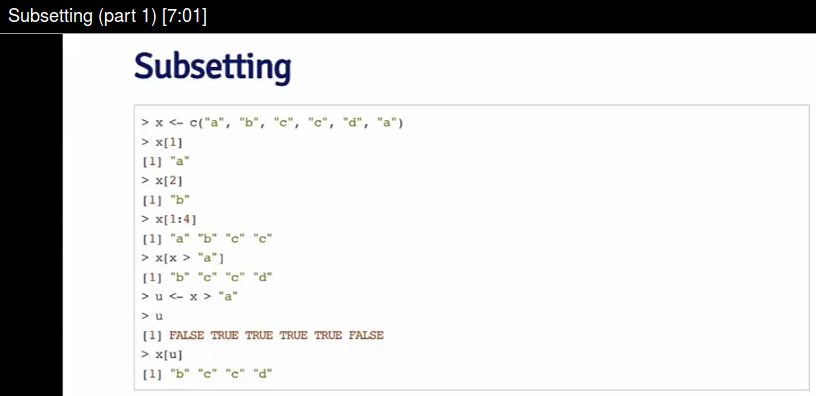
\includegraphics[width=0.45\textwidth]{01_rprogramming/pics/subset1}}
\subfigure[]{\label{fig:}
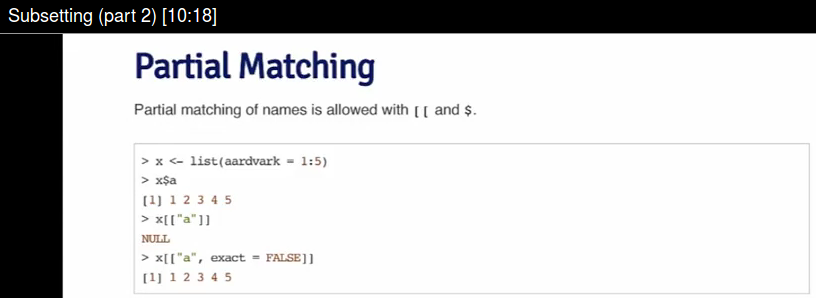
\includegraphics[width=0.45\textwidth]{01_rprogramming/pics/subset2}}
\caption{}
\end{center}\end{figure}

\begin{figure}[htb]\begin{center}
\subfigure[]{\label{fig:}
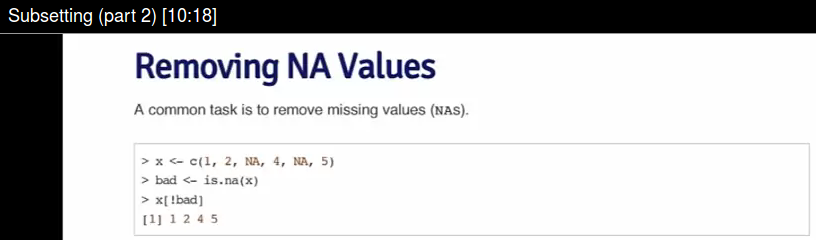
\includegraphics[width=0.45\textwidth]{01_rprogramming/pics/subset3}}
\subfigure[]{\label{fig:}
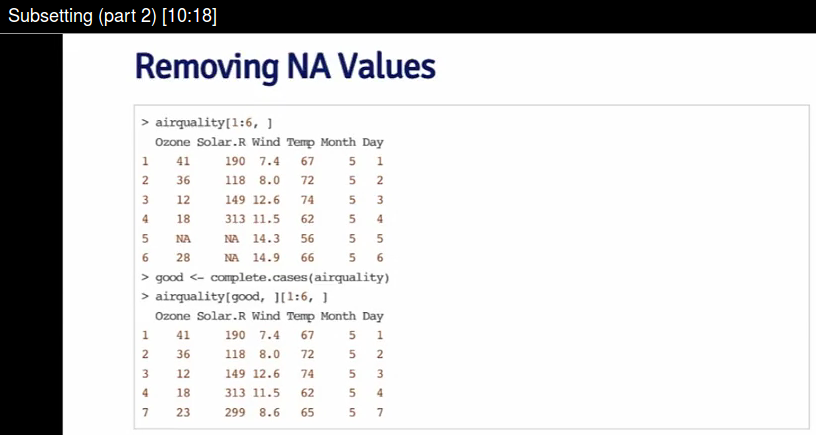
\includegraphics[width=0.45\textwidth]{01_rprogramming/pics/subset4}}
\caption{}
\end{center}\end{figure}

\begin{figure}[htb]\begin{center}
\subfigure[]{\label{fig:}
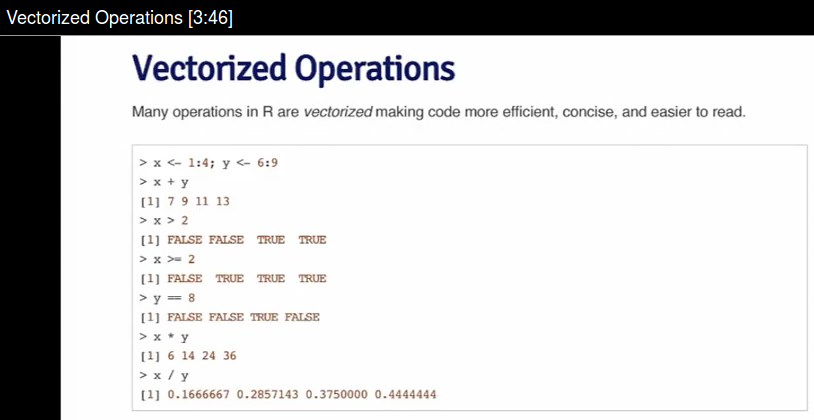
\includegraphics[width=0.45\textwidth]{01_rprogramming/pics/subset5}}
\subfigure[]{\label{fig:}
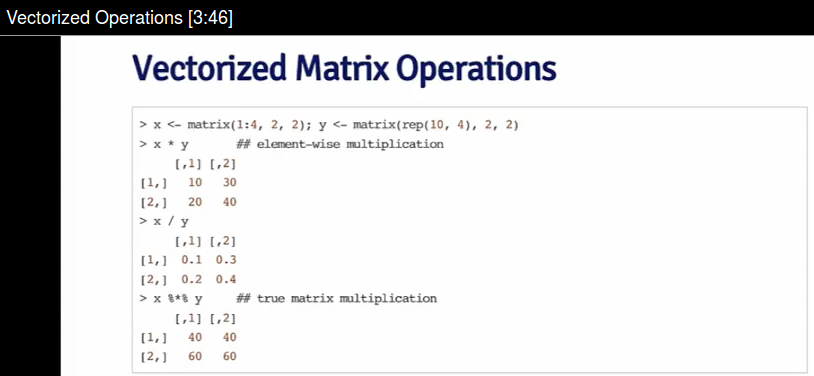
\includegraphics[width=0.45\textwidth]{01_rprogramming/pics/subset6}}
\caption{}
\end{center}\end{figure}

\begin{figure}[htb]\begin{center}
\subfigure[]{\label{fig:}
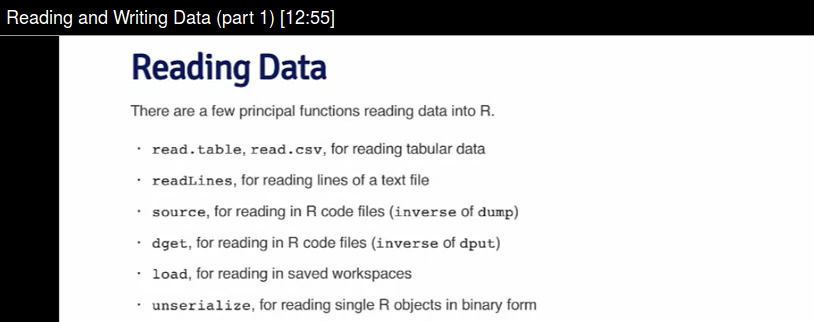
\includegraphics[width=0.45\textwidth]{01_rprogramming/pics/readingdata1}}
\subfigure[]{\label{fig:}
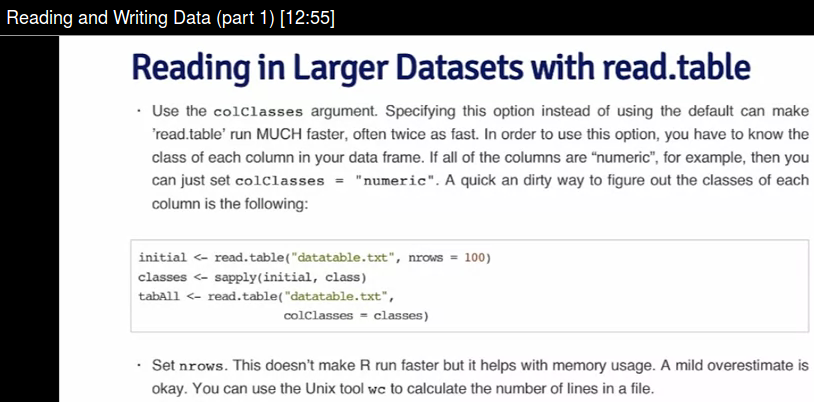
\includegraphics[width=0.45\textwidth]{01_rprogramming/pics/readingdata2}}
\caption{}
\end{center}\end{figure}

\begin{figure}[htb]\begin{center}
\subfigure[]{\label{fig:}
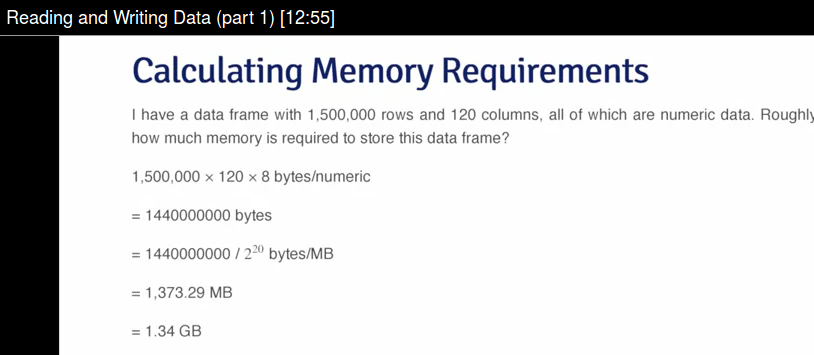
\includegraphics[width=0.45\textwidth]{01_rprogramming/pics/readingdata3}}
\subfigure[]{\label{fig:}
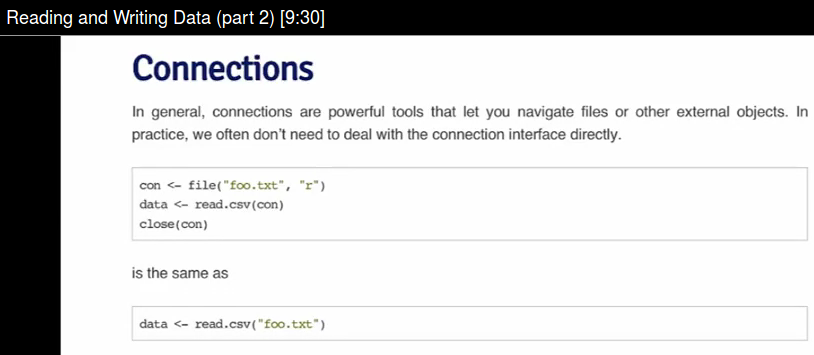
\includegraphics[width=0.45\textwidth]{01_rprogramming/pics/readingdata4}}
\caption{}
\end{center}\end{figure}

\begin{figure}[htb]\begin{center}
\subfigure[]{\label{fig:}
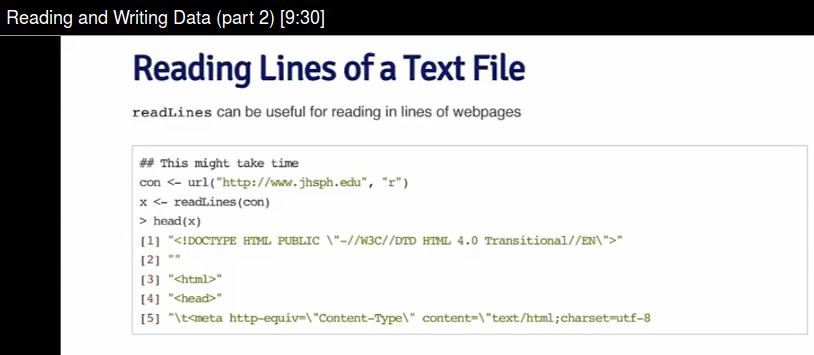
\includegraphics[width=0.45\textwidth]{01_rprogramming/pics/readingdata5}}
\subfigure[]{\label{fig:}
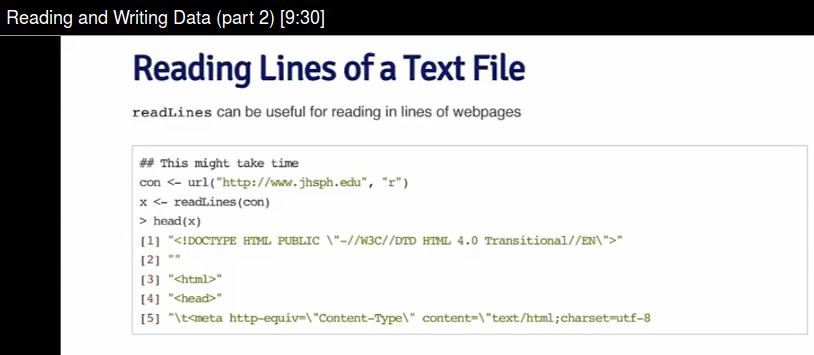
\includegraphics[width=0.45\textwidth]{01_rprogramming/pics/readingdata5}}
\caption{}
\end{center}\end{figure}
